\documentclass{article}
\usepackage{tikz}
\usepackage{float}
\usepackage{enumerate}
\usepackage{amsmath}
\usepackage{amsthm}
\usepackage{bm}
\usepackage{indentfirst}
\usepackage{siunitx}
\usepackage[utf8]{inputenc}
\usepackage{graphicx}
\graphicspath{ {Images/} }
\usepackage{float}
\usepackage{mhchem}
\usepackage{chemfig}
\allowdisplaybreaks

\title{6.041 Problem Set 13}
\author{Robert Durfee - R02}
\date{December 5, 2018}

\begin{document}

\maketitle

\section*{Problem 1}

\subsection*{Part A}

\begin{center}
    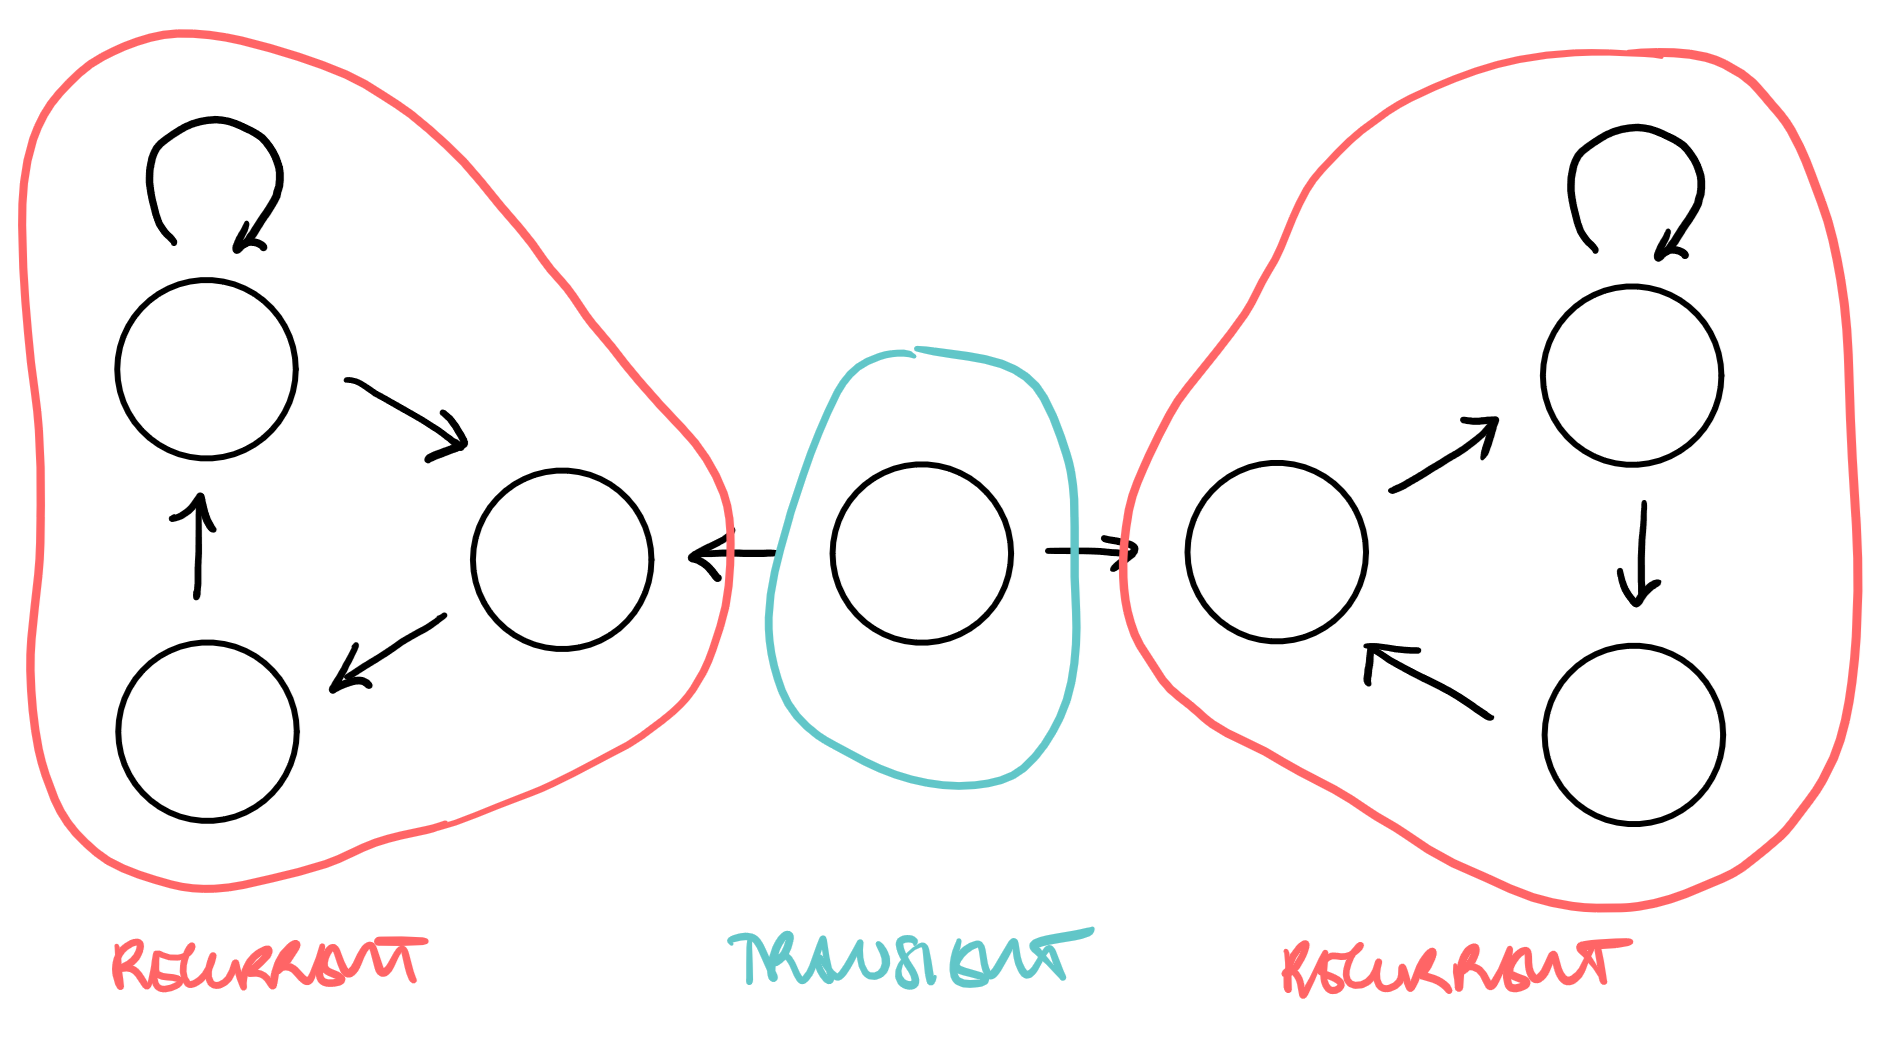
\includegraphics[scale=0.25]{Images/P1A.PNG}
\end{center}

\subsubsection*{Part I}

False. There are two recurrent classes. As a result, the steady states depend
on the initial $i$.

\subsubsection*{Part II}

False. Part I is false.

\subsection*{Part B}

\begin{center}
    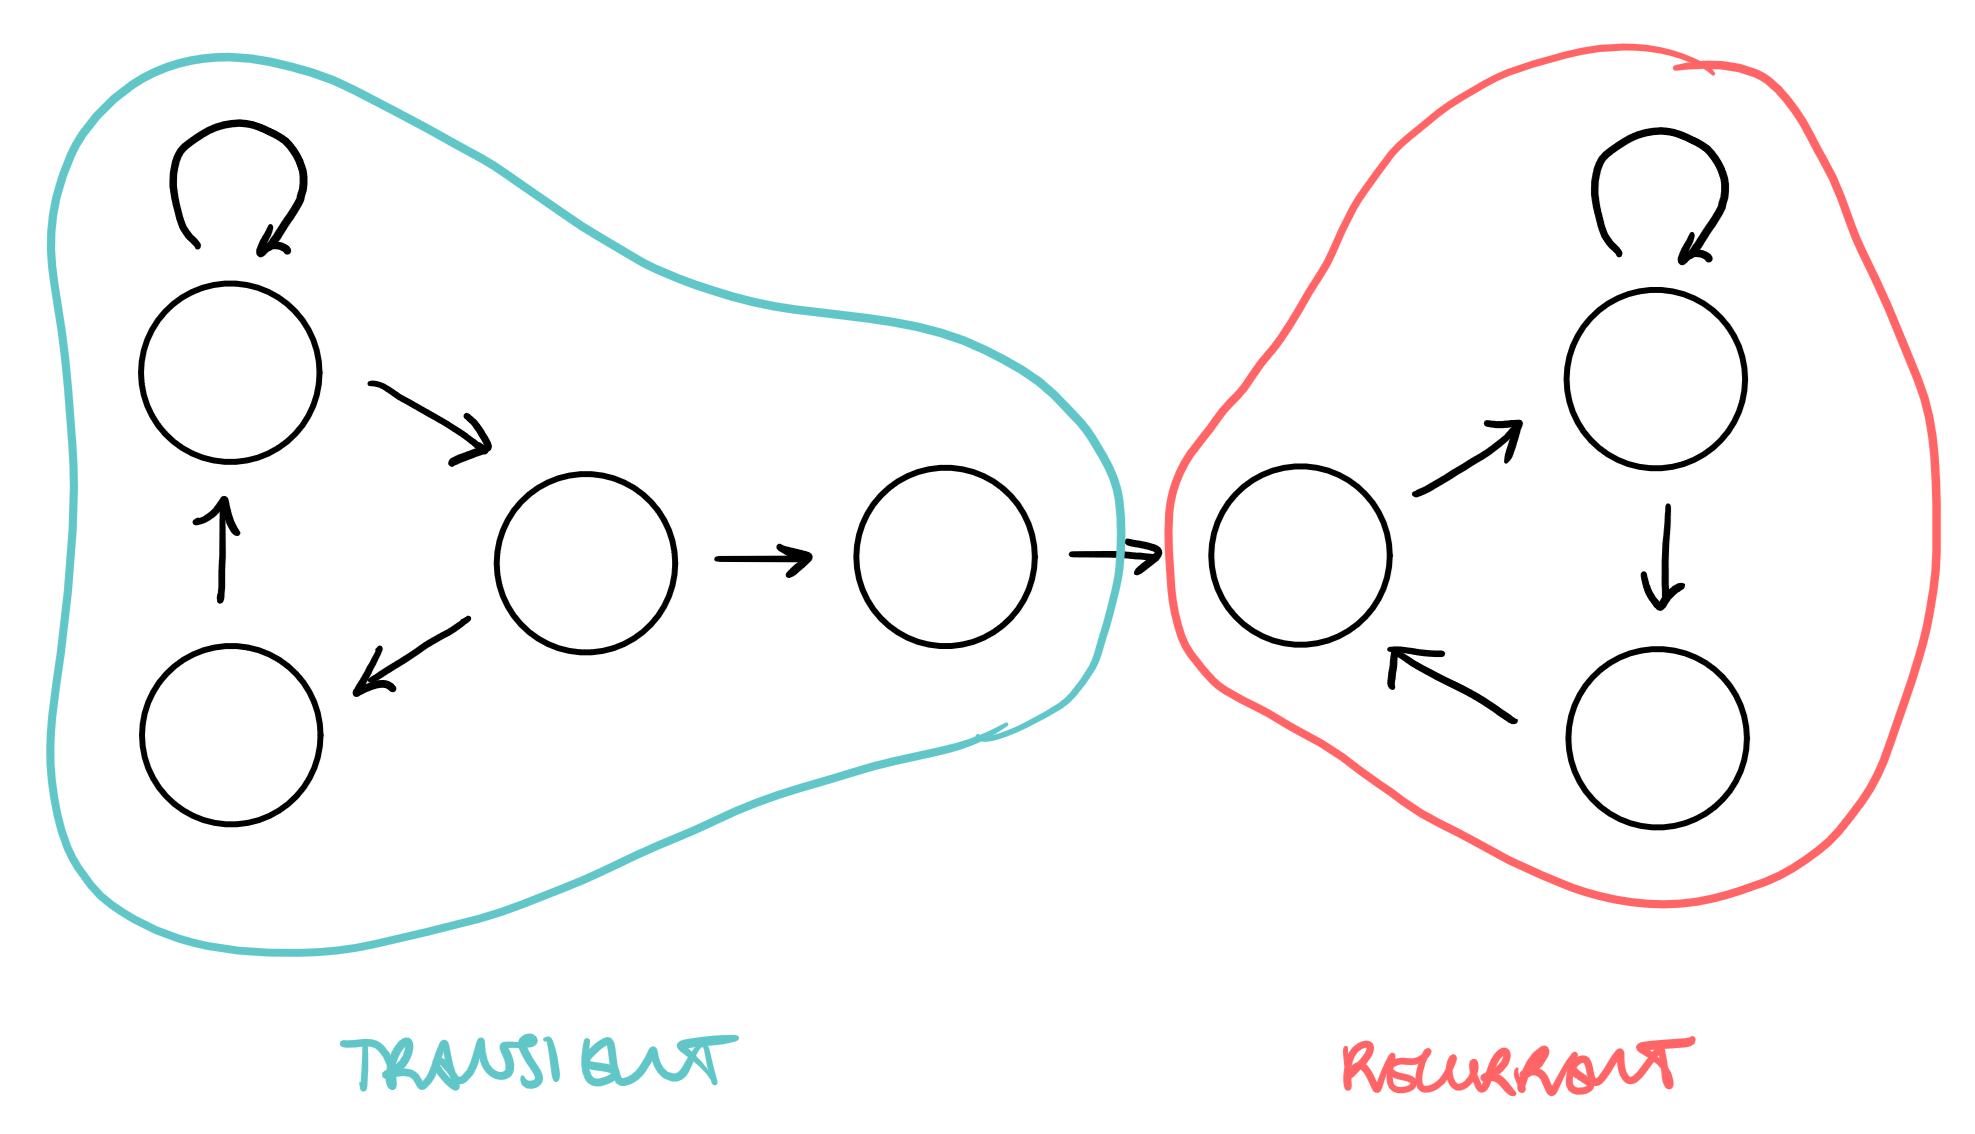
\includegraphics[scale=0.25]{Images/P1B.PNG}
\end{center}

\subsubsection*{Part I}

True. There is only one recurrent class. This class is also aperiodic as
there is a self-transition.

\subsubsection*{Part II}

False. There are transient states which, as $n \longrightarrow \infty$,
approaches a steady-state of zero.

\subsection*{Part C}

\begin{center}
    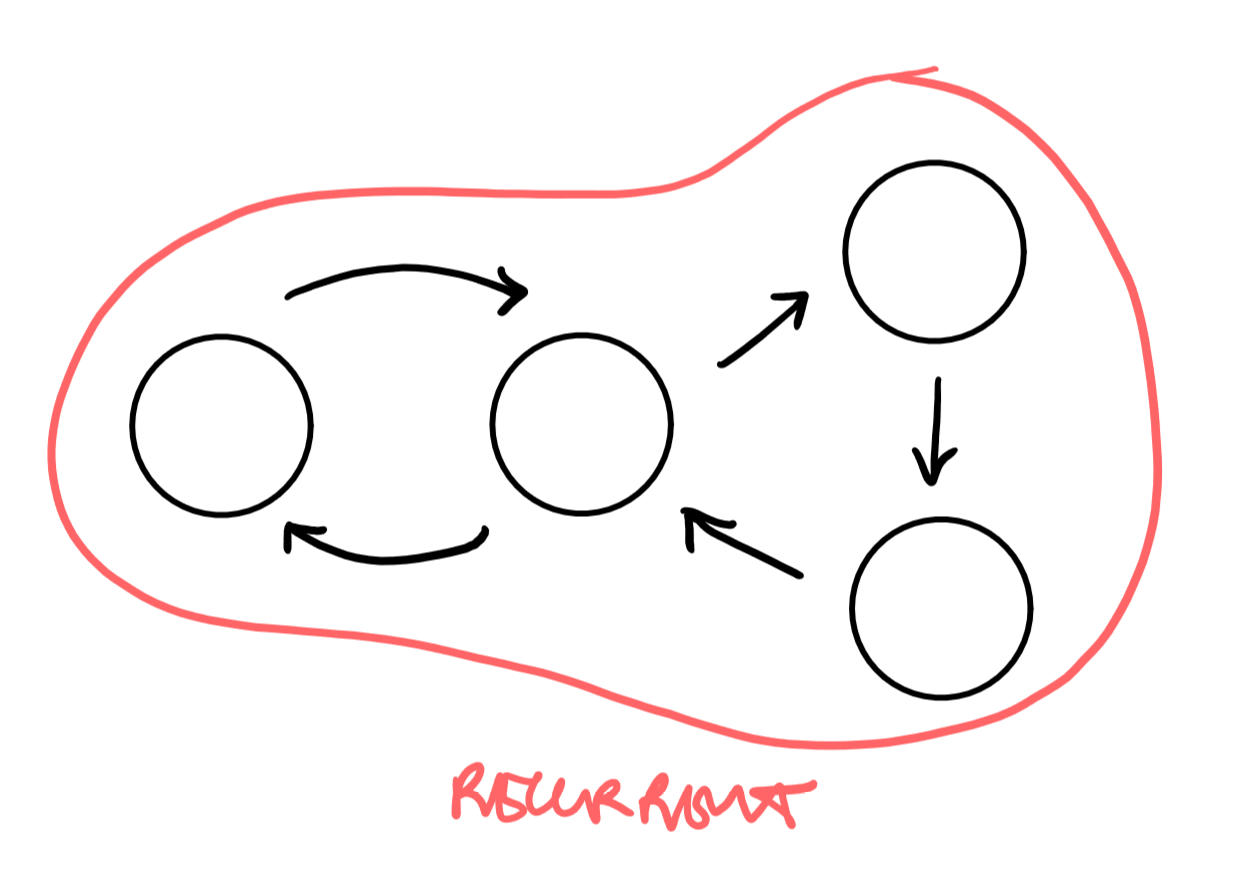
\includegraphics[scale=0.25]{Images/P1C.PNG}
\end{center}

\subsubsection*{Part I}

True. There is one recurrent class. This class is also aperiodic as the GCD
of all loops is $1$.

\subsubsection*{Part II}

True. There are no transient states.

\section*{Problem 2}

\subsection*{Part A}

\begin{center}
    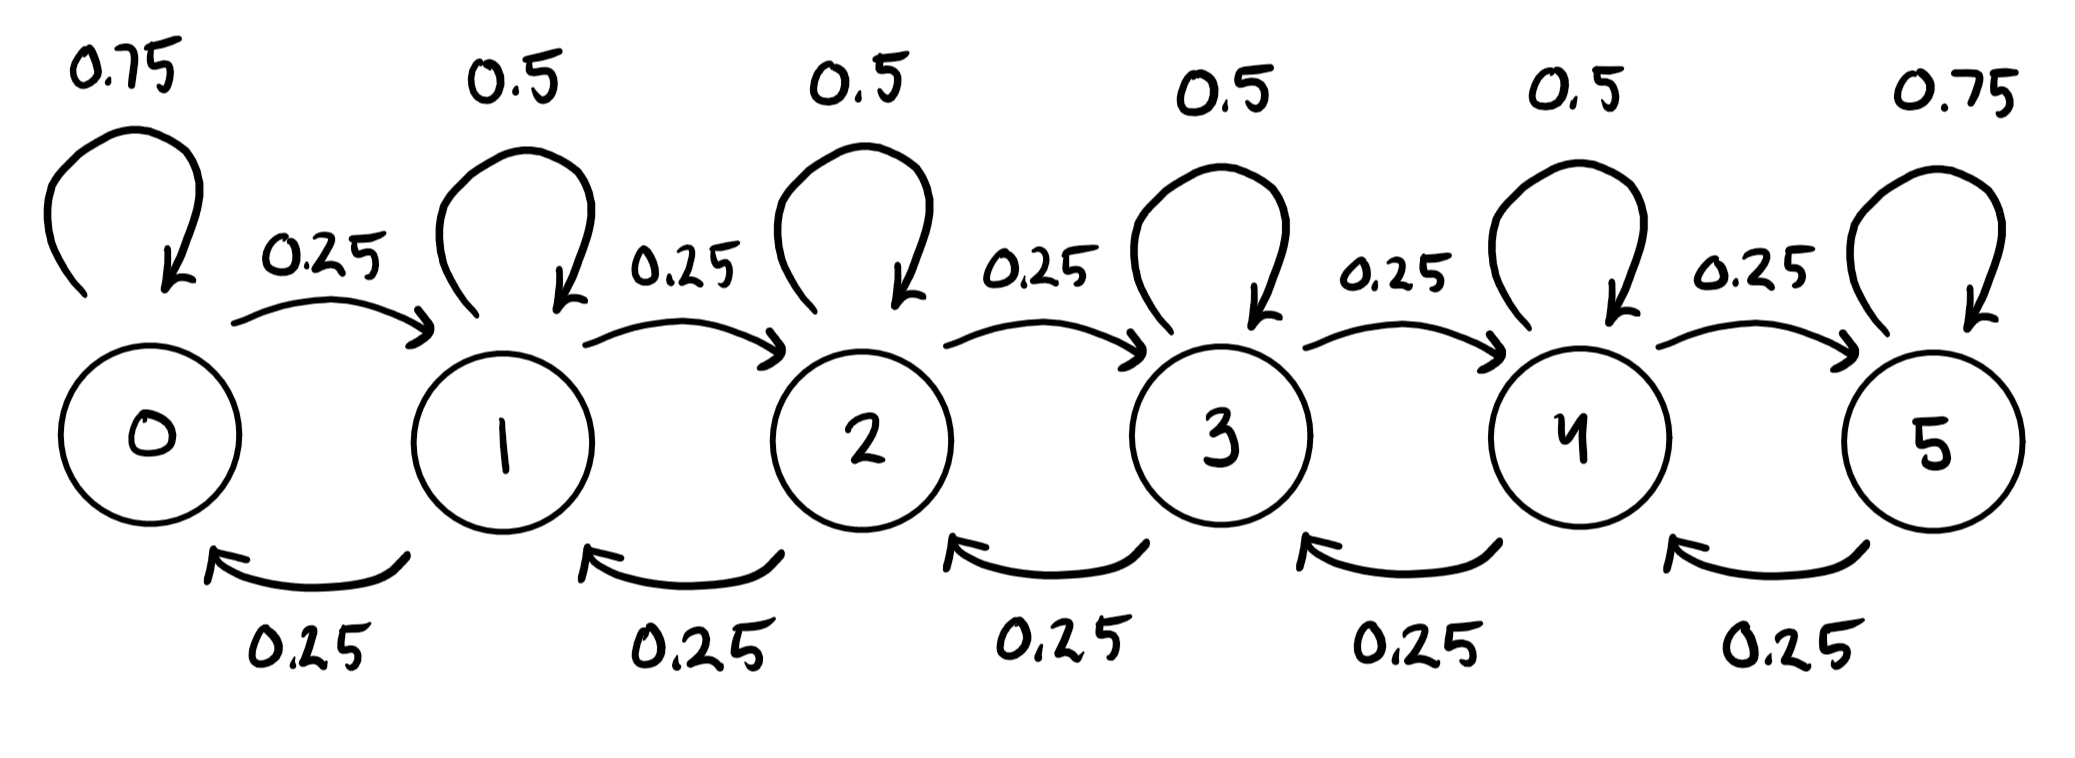
\includegraphics[scale=0.25]{Images/P2A.PNG}
\end{center}

The transition probabilities are shown above. This comes from realizing that
there are only four possible options for Oscar:
\begin{itemize}
  \item He can go from the front door to the front door. In which case the
  number of shoes at both doors will remain the same.
  \item He can go from the front door to the back door. In which case the
  number of shoes at the front door will decrease by one and the number of
  shoes at the back door will increase by one (so long as Oscar's not
  barefoot).
  \item He can go from the back door to the front door. In which case the
  number of shoes at the back door will decrease by one and the number of 
  shoes at the front door will increase by one (so long as Oscar's not 
  barefoot).
  \item He can go from the back door to the back door. In which case the
  number of shoes at both doors will remain the same.
\end{itemize}

\subsection*{Part B}

The steady-state probability that Oscar runs barefoot is the steady-state
probability of being in state zero. This steady-state can be determined using
the detailed balancing equations as this process is a birth-death process.
$$ 0.25 \cdot \pi_i = 0.25 \cdot \pi_{i + 1}\quad \forall i \in \{0, \ldots,
4\} $$
$$ \sum_{i = 0}^{5} \pi_i = 1 $$
Solving this system of equations yields the following steady states,
$$ \pi_0 = \pi_1 = \ldots = \pi_5 = 1/6 $$
Therefore, the steady-state probability of Oscar running barefoot is $1/6$.

\section*{Problem 3}

\subsection*{Part A}

The probablity $P(X_2 = 2 \mid X_0 = 1)$ is given by
$$ r_{12}(2) = \sum_k r_{1k}(1) p_{k2} $$
Given that $r_{ij}(1) = p_{ij}$, this simplifies,
$$ r_{12}(2) = \sum_k p_{1k} \cdot p_{k2} $$
Since there are only two ways to get to state two,
$$ r_{12}(2) = p_{11} \cdot p_{12} + p_{12} \cdot p_{22} = 0.6 \cdot 0.4 +
0.4 \cdot 0.5 = 0.44 $$

\subsection*{Part B}

The detailed balancing equations can once again be used becase this is a
birth-death process.
$$ 0.4 \cdot \pi_1 = 0.2 \cdot \pi_2 $$
$$ 0.3 \cdot \pi_2 = 0.1 \cdot \pi_3 $$
$$ \pi_1 + \pi_2 + \pi_3 = 1 $$
Solving this system of equations yields the steady-states,
$$ \pi_1 = 1/9,\quad \pi_2 = 2/9,\quad \pi_3 = 2/3 $$

\subsection*{Part C}

As $n \longrightarrow \infty$, right transitions will happen when,
$$ 1 \rightarrow 2: \pi_1 \cdot p_{12} = 1/9 \cdot 2/5 = 0.0444 $$
$$ 2 \rightarrow 3: \pi_2 \cdot p_{23} = 2/9 \cdot 3/10 = 0.0667 $$
Combining these using the Law of Total Probability,
$$ \lim_{n\rightarrow\infty} P(Y_n = 1) = 0.0444 + 0.0667 = 1/9 $$

\subsection*{Part D}

No, the sequence $Y_1, Y_2, \ldots$ is not a Markov chain. Since the
transition probabilities between the states $\{-1, 0, +1\}$ depends on more
than just the state, this cannot be a Markov chain.

\subsection*{Part E}

Using Baye's Rule,
\begin{align*}
  P(X_{n - 1} = 1 \mid Y_n = 1) &= \frac{P(X_{n - 1} = 1) P(Y_n = 1 \mid X_{n
  - 1} = 1)}{P(Y_n = 1)} \\
  &= \frac{\pi_1 \cdot p_{12}}{\pi_1 \cdot p_{12} + \pi_2 \cdot p_{23}} \\
  &= \frac{1/9 \cdot 2/5}{1/9} \\
  &= \frac{2}{5}
\end{align*}

\subsection*{Part G}

The sequence $X_1, X_2, \ldots$ does not converge to a constant. Even after
the Markov chain reaches a steady-state, since it is a single recurrent class
with no transient classes, the states will always be changing.

\subsection*{Part H}

The sequence $Z_1, Z_2, \ldots$ does converge to a constant. Although the
$X$'s will continuously change, they will eventually reach the $3$-state as
it is in the recurrent class. There are no higher states so the maximum of
all previous $X$'s will eventually converge to $3$ and stay there.

\section*{Problem 4}

Consider the following Markov chain that represents the given situation.

\begin{center}
    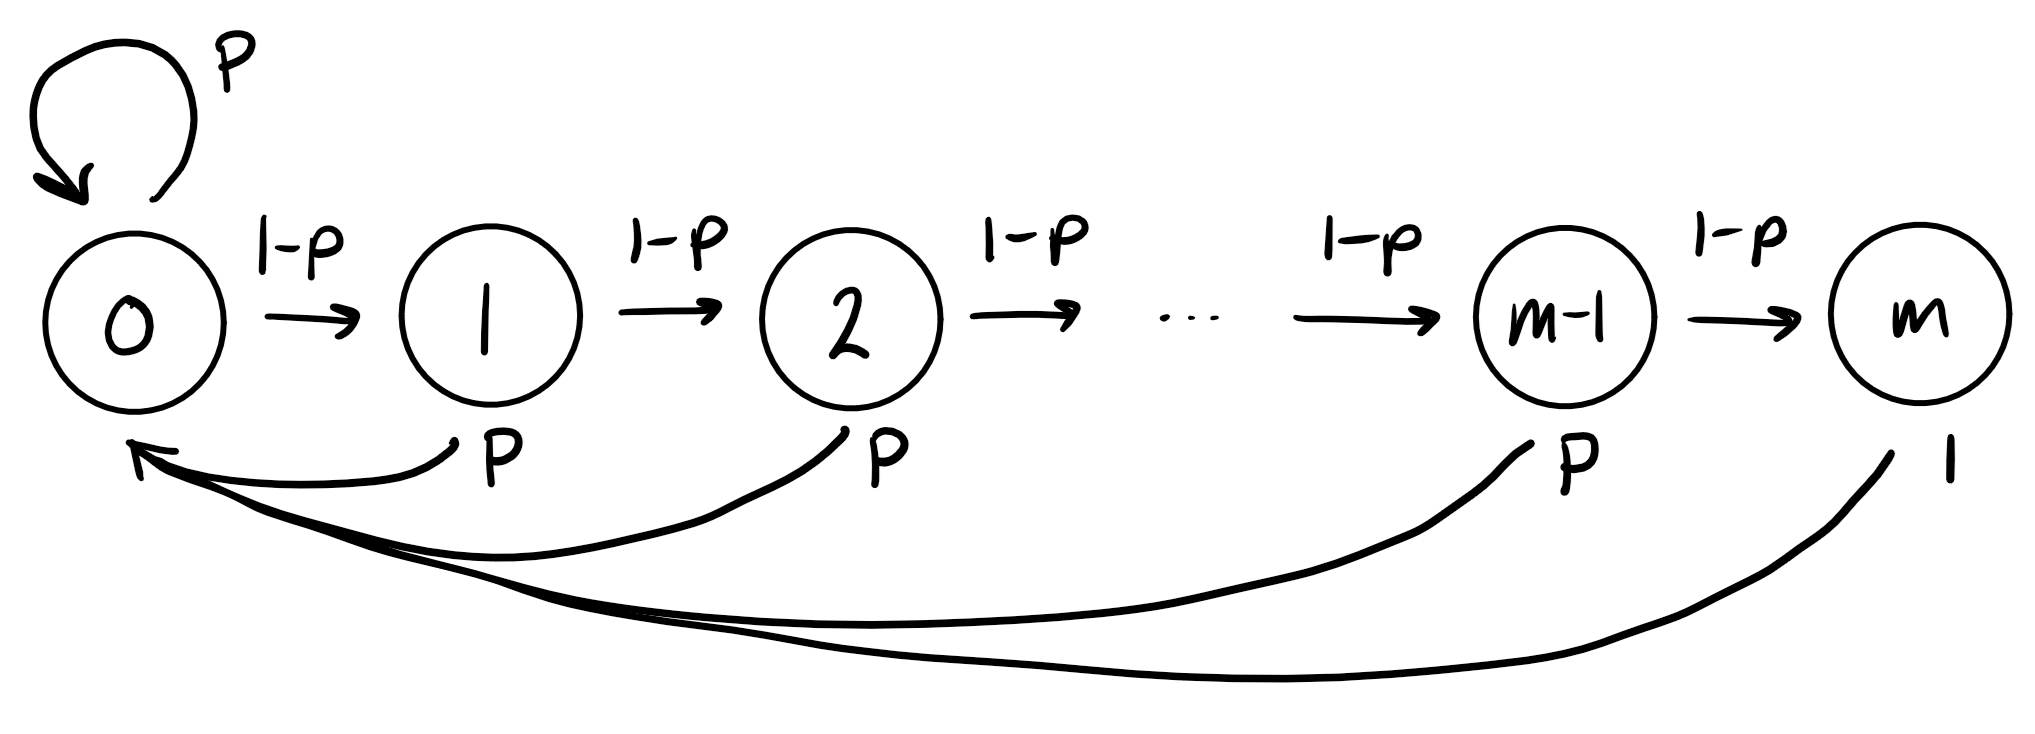
\includegraphics[scale=0.25]{Images/P4.PNG}
\end{center}

To calculate the steady-state, first look at states $1$ through $m$,
\begin{align*}
  \pi_1 &= (1 - p) \pi_0 \\
  \pi_2 &= (1 - p) \pi_1 \\
  &\vdots \\
  \pi_m &= (1 - p) \pi_{m - 1}
\end{align*}
Because of this recursion, each of these states can be written as,
$$ \pi_i = (1 - p)^i \pi_0\quad \forall i \in \{1, \ldots, m\} $$
Using the normalization condition,
$$ \sum_{k=0}^{m} \pi_k = 1$$
The steady-state for state zero can be written in closed form,
$$ 1 = \pi_0 \sum_{k=0}^{m} (1 - p)^k = \frac{\pi_0 (p(1 - p)^m - (1 - p)^m +
1)}{p} $$
Solving for $\pi_0$,
$$ \pi_0 = \frac{p}{p(1 - p)^m - (1 - p)^m + 1} $$

\end{document}